% Chapter 5
\chapter{Resultados}
\label{Capítulo5}

\begin{flushright}
\textit{``Newton's third law. You've got to leave something behind''} \\[0.5em]
--- Cooper, \textit{Interstellar}
\end{flushright}

Os testes foram realizados com o objetivo de validar a implementação do \acrshort{lare} e verificar se os resultados obtidos correspondem aos esperados. Como forma de uniformizar conceitos, apesar de tanto as experiências desenvolvidas no \acrshort{lare} como as realizadas na ``placa branca'' serem reais, designar-se-ão os testes efetuados na ``placa branca'' como experiências práticas ou valores práticos.

Sendo assim, a confrontação dos resultados obtidos no \acrshort{lare} foi efetuada com recurso às experiências práticas, ao \href{https://www.multisim.com}{\textit{MultisimLive}} e aos valores teóricos previamente descritos na Secção \ref{sec:experiencias}. Para a análise dos resultados, serão apresentados um ou dois exemplos representativos por tipo de experiência, sendo que os restantes são obtidos de forma análoga. No caso específico da Lei de \textit{Ohm}\footnote{Uma vez que a versão grátis \textit{online} do \textit{MultisimLive} não permite realizar a análise continua - \textit{dc sweep} - esta análise fez-se utilizando o \href{https://www.circuitlab.com/}{CircuitLab}}, há ainda a possibilidade de verificar os valores com recurso a um multímetro de bancada. As experiências podem ser realizadas com diferentes combinações e configurações:

\begin{itemize}
	\item \textbf{Lei de \textit{Ohm}}: três opções de estudo de resistências;
	\item \textbf{Rectificadores}: quatro combinações possíveis de resistências e condensadores para cada rectificador;
	\item \textbf{Filtros}: duas combinações possiveis de resistências e condensadores para cada filtro.
\end{itemize}

\section{Lei de \textit{Ohm}}
\label{sec:resultados_lei_de_ohm}
O objetivo desta experiência é determinar o valor de uma determinada resistência através do cálculo do declive da recta obtida no gráfico da tensão em função da corrente apresentado na Figura \ref{fig:graphohm} e, assim, confirmar a Lei de \textit{Ohm}.

\subsection{Resultados experimentais}
\label{sec:resultados_praticosOHM}
No \acrshort{lare} o utilizador efectua cinco medições de cada grandeza (tensão e corrente), para uma das três resistências disponíveis. Na Figura \ref{fig:resultados_medicoes_1k} está representado o resultado de um par de medições para uma resistência de \SI{1}{\kilo\ohm}. As restantes medições, em intervalos de \SI{1}{\volt} até \SI{5}{\volt}, são obtidas de forma análoga.

\begin{figure}[hbtp]
	\centering
	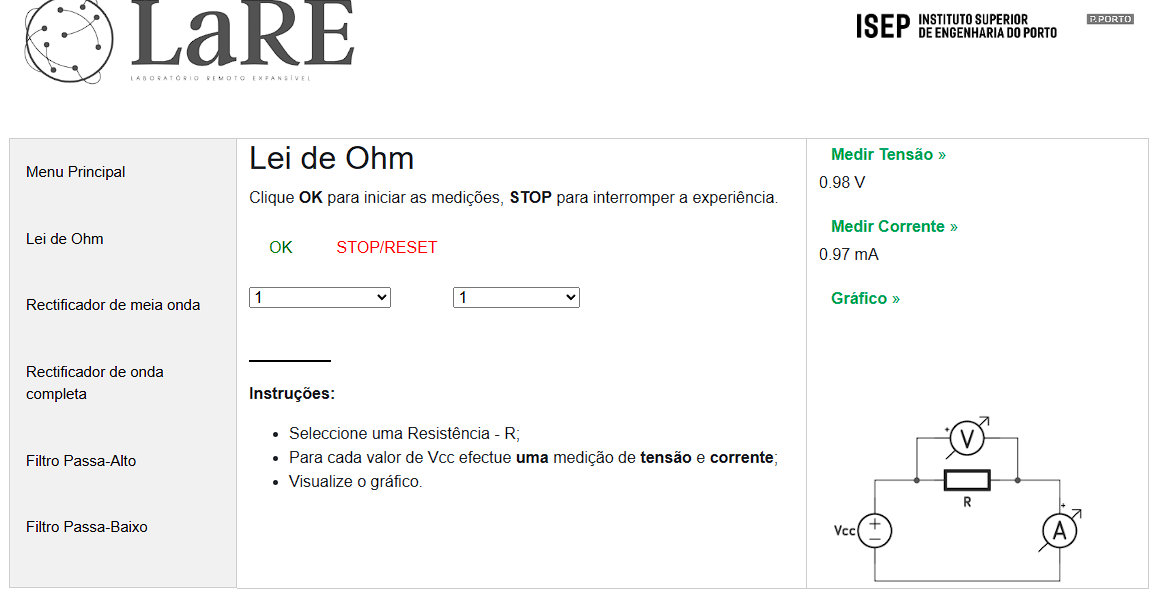
\includegraphics[width=0.6\textwidth]{figures/resultados_medicoes_ohm.png}
	\caption{Medição prática}
	\label{fig:resultados_medicoes_1k}
\end{figure}

O valor real da resistência, obtida por medição directa, é de \SI{998}{\ohm}, estando dentro da tolerância que é de $\pm$5\%. O erro associado aos instrumentos de medição pode ser considerado desprezável. De acordo com as especificações do modelo \textit{VB-8012}\cite{datasheetvb8012}, a precisão para medições de tensão em corrente contínua é:

\begin{itemize}
	\item Escala de \SI{1}{\volt}
	\begin{itemize}
		\item Precisão garantida (1 ano): $\pm$(0.015\% da leitura $\pm$ 0.005\% da faixa)
	\end{itemize}
\end{itemize}

Estes valores indicam que, para uma leitura de \SI{1}{\volt}, o erro máximo estimado devido à precisão do instrumento seria de, aproximadamente $\pm$\SI{0.0002}{\volt}, ou seja, $\pm$\SI{0.2}{\milli\volt}. Portanto, a diferença entre a tensão fornecida pela fonte — \SI{1}{\volt} — e os valores medidos — \SI{0.98}{\volt} e \SI{0.97}{\milli\ampere} — deve-se, principalmente, à tolerância da resistência utilizada. Assim, conclui-se que os valores medidos se encontram dentro dos limites expectáveis, sendo perfeitamente aceitáveis face às tolerâncias envolvidas.

O gráfico \textit{U vs I}, obtido para esta resistência é apresentado na Figura \ref{fig:grafico_LaRE_1k}. O declive da recta, que representa a resistência, foi calculado e comparado com o valor real da resistência. 

\begin{figure}[hbtp]
	\centering
	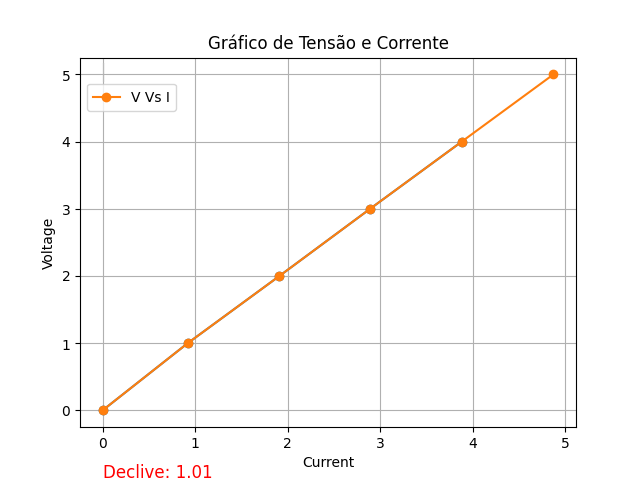
\includegraphics[width=0.6\textwidth]{figures/ohm_graph.png}
	\caption{Gráfico da Lei de \textit{Ohm} - \SI{1}{\kilo\ohm} - \acrshort{lare}}
	\label{fig:grafico_LaRE_1k}
\end{figure}

O erro relativo entre o valor teórico e o valor obtido no \acrshort{lare}, pode ser calculado através da Equação \ref{eq:errorelativo}:

\begin{equation} \label{eq:errorelativo}
	\text{Erro Relativo} = \frac{|R_{real} - R_{obtido}|}{R_{real}} \times 100
\end{equation}

O erro relativo obtido é de, aproximadamente, \SI{1.2}{\percent}, sendo um valor perfeitamente aceitável.

Os resultados da experiência prática, efectuados com a mesma resistência utilizada no \acrshort{lare}, estão representados na Tabela \ref{Table:valoresexperimentaisohm}.

\begin{table}[htb]
	\centering
	\caption{Valores práticos - Lei de \textit{Ohm}} 
	\label{Table:valoresexperimentaisohm}
	\begin{tabular}{lcc}
		\toprule
		Tensão (V)& Corrente (mA) & Resistência (\SI{}{\kilo\ohm}) \\
		\midrule
		$0.998$ & 0.998 & 1  \\
		\midrule
		 $1.99$ & 1.99  & 1  \\
		 \midrule
		 $2.99$ & 2.99  & 1  \\
		 \midrule
		 $3.99$ & 3.99  & 1  \\
		 \midrule
		 $4.99$ & 4.99  & 1  \\
		\bottomrule
	\end{tabular}
\end{table}

Estes valores foram obtidos com recurso ao \acrshort{virtualbench} e demonstram que o valor da resistência, que corresponde ao declive da recta é constante, o que confirma a Lei de \textit{Ohm}. A partir da Equação \ref{eq:errorelativo}, o valor do erro relativo é inferior a \SI{1}{\percent}. 

Ainda assim e como forma de complementar a análise dos resultados, foram efectuados testes com o \href{https://www.multisim.com}{\textit{Multisim}}. A Figura \ref{fig:multisimOHM} mostra o gráfico obtido.

\begin{figure}[hbtp]
	\centering
	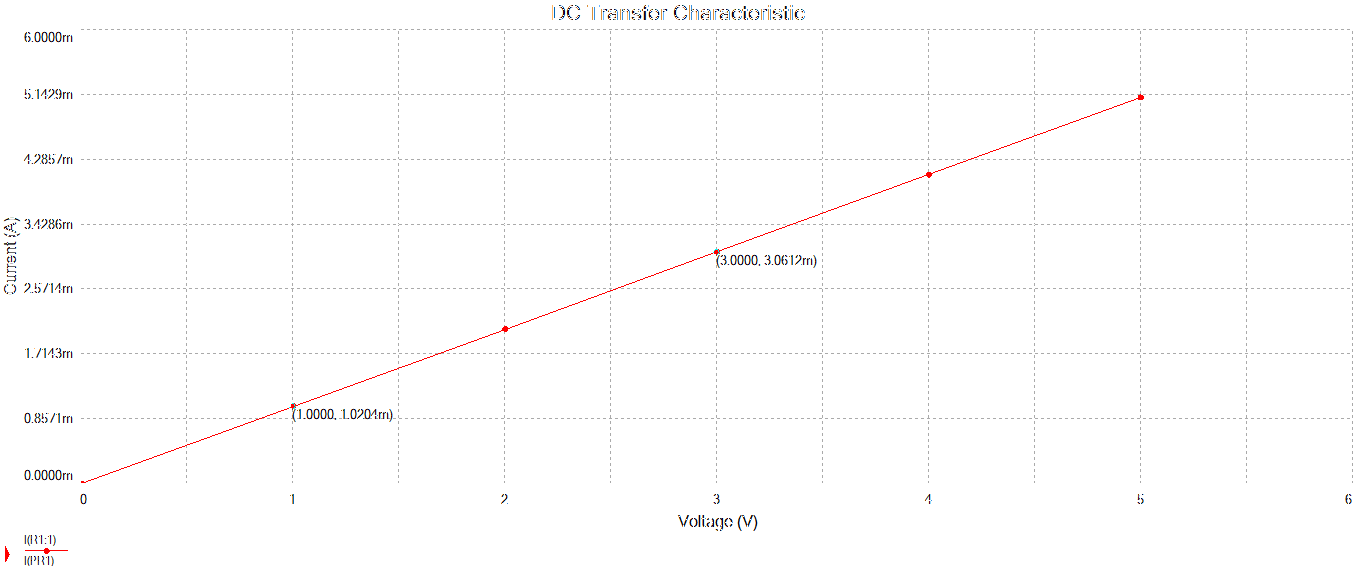
\includegraphics[width=0.6\textwidth]{figures/OHM_resultado_multisim.png}
	\caption{Multisim - Lei de \textit{Ohm}}
	\label{fig:multisimOHM}
\end{figure}

Analisando os valores é possível calcular o declive da recta, dado pela Equação \ref{eq:declive}:

\begin{equation} \label{eq:declive}
	\text{m} = \frac{y_{b} - y_{a}}{x_{b} - x_{a}}
\end{equation}

O valor do declive, correspondente à resistência, obtido para estes simuladores é de $m_\text{{multisim}} \approx{0.980}$. Tendo em conta que a escala do eixo do $y$ está representada em \SI{}{\milli\ampere}, os valores das resistências surgem expressos em \SI{}{\kilo\ohm}, isto é, $R_\text{{multisim}} = \SI{0.980}{\kilo\ohm}$. Assim, aplicando a Equação~\ref{eq:errorelativo} obtém-se um erro relativo inferior a \SI{1}{\percent}.

Verifica-se, através da análise dos gráficos, que os dados obtidos com o \acrshort{lare} estão em concordância com os resultados simulados e com os valores práticos.

\section{Rectificadores}
\label{sec:resultados_rectificadores}
As duas experiências foram implementadas com o objectivo de estudar e avaliar a tensão de \textit{ripple} nos circuitos rectificadores de meia onda e onda completa, considerando as quatro combinações possíveis dos pares resistência/condensador. As formas de onda esperadas estão representadas na Figura \ref{fig:formadeonda_MO} e Figura \ref{fig:formadeonda_OC} sendo os valores teóricos da tensão de \textit{ripple} determinados pela Equação \ref{eq:vripplecompleta} e pela Equação \ref{eq:vrippleOC} - (ou Equação \ref{eq:vripple}). Os utilizadores podem escolher uma das quatro combinações de resistência e condensador, sendo que no caso do rectificador de meia onda podem fazer variar a frequência entre \SI{50}{\hertz} e \SI{2000}{\hertz} mas no caso do rectificador de onda completa a frequência é de \SI{50}{\hertz}. Em ambas as experiências, os exemplos em análise far-se-ão com os seguintes valores: $R=\SI{2.2}{\kilo\ohm}$, $C=\SI{100}{\micro\farad}$, $v_{in}=\SI{6.6}{\volt}$ e $f=\SI{50}{\hertz}$.

\subsection{Resultados experimentais [meia onda]}
\label{sec:resultados_RectificadoresMeiaOnda}
Para se determinar qual expressão a usar para calcular a tensão de \textit{ripple}, é necessário verificar a condição descrita na Equação \ref{eq:verificarcondicao}:

\begin{equation} \label{eq:verificarcondicao}
	RC >> \dfrac{1}{f}
\end{equation}

\begin{equation}
	\SI{2.2}{\kilo\ohm} * \SI{100}{\micro\farad} >> \dfrac{1}{100}
\end{equation}

Uma vez que esta condição se verifica, a expressão a utilizar para calcular a tensão de \textit{ripple} teórica pode ser dada pela sua aproximação, representada pela Equação \ref{eq:vripple}. O resultado obtido está representado na Equação \ref{eq:vripplecalculado}:

\begin{equation} \label{eq:vripplecalculado}
	U_{ripple} = \frac{\SI{6.6}{\volt}-\SI{0.7}{\volt}}{\SI{50}{\hertz}*\SI{2.2}{\kilo\ohm}*\SI{100}{\micro\farad}} \approx \SI{536.36}{\milli\volt}
\end{equation}

A Figura \ref{fig:ripplelaremeiaonda} apresenta a forma de onda da tensão de saída e o valor da tensão de \textit{ripple} obtido no \acrshort{lare}, que foi de \SI{420}{\milli\volt}.

\begin{figure}[hbtp]
	\centering
	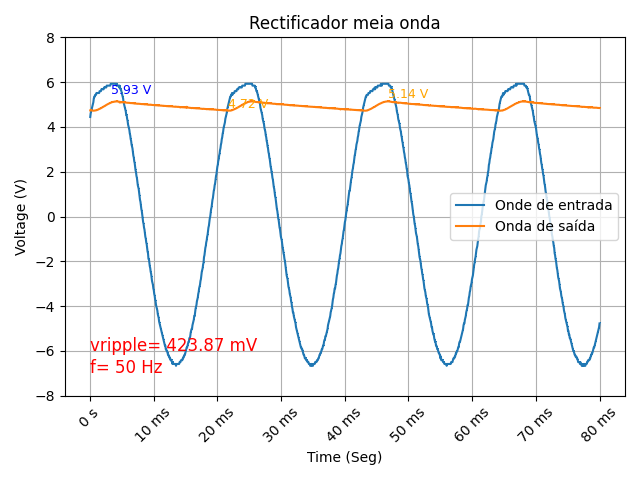
\includegraphics[width=0.5\textwidth]{figures/ripple_lare_MO-2k2-100uF.png}
	\caption{Tensão de \textit{ripple} no \acrshort{lare} - meia onda}
	\label{fig:ripplelaremeiaonda}
\end{figure}

As Figuras \ref{fig:realmeiaonda} e \ref{fig:multisimmeiaonda} representam, respectivamente, os resultados práticos e simulados. A tensão de ripple medida foi de \SI{481}{\milli\volt} e \SI{490.98}{\milli\volt}, respectivamente.

\begin{figure}[hbtp]
	\centering%
		\centering
		\subfloat[\centering Circuito prático\label{fig:realmeiaonda}]{{\includegraphics[width=6.3cm]{figures/ripple_práctica_MO-2k2-100uF.png} }}%
		\qquad
		\subfloat[\centering Simulação \textit{multisim}\label{fig:multisimmeiaonda}]{{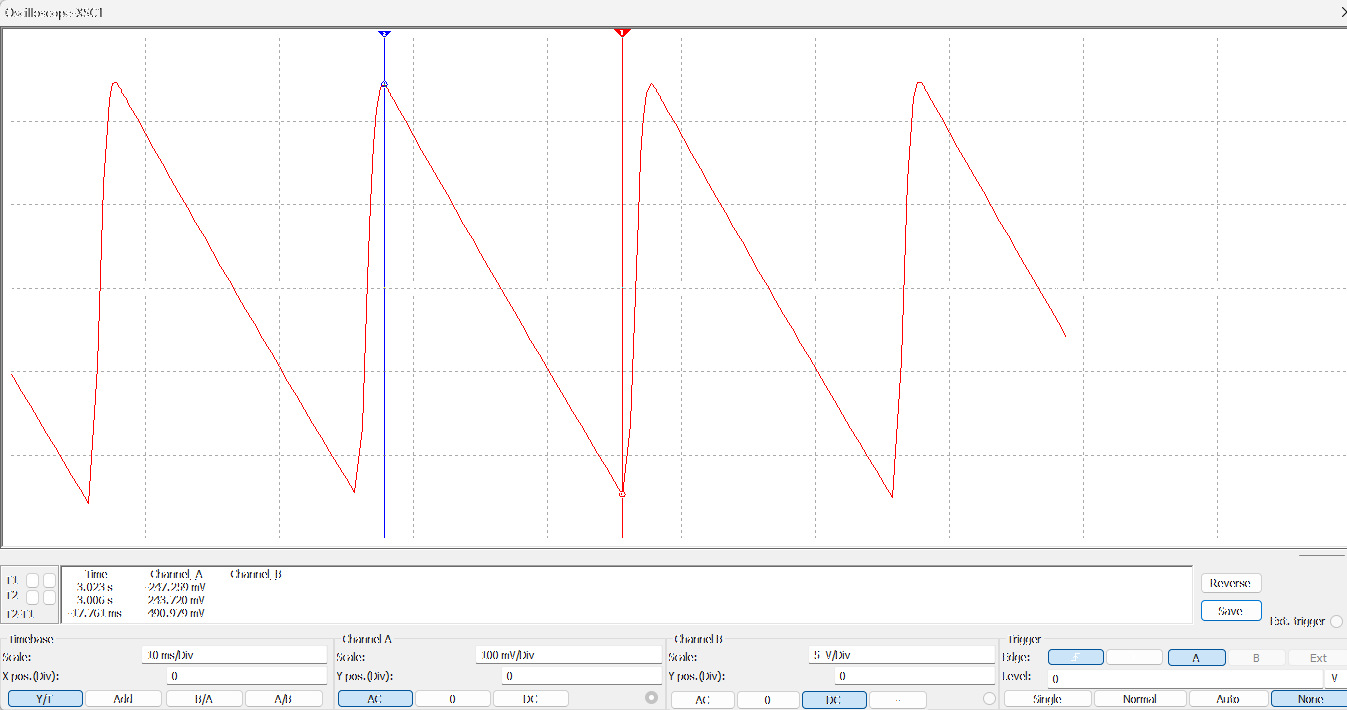
\includegraphics[width=6.3cm]{figures/ripple_multisim_MO-2k2-100uFALT.png} }}%
		\caption{Valores experimentais e simulados - tensão de \textit{ripple}}%
		\label{fig:simulacaoripple}%
	\end{figure}

Os erros relativos obtidos foram de \SI{20.1}{\percent} no \acrshort{lare}, \SI{10.32}{\percent} no circuito prático e \SI{8.46}{\percent} na simulação. Esta discrepância relativamente ao valor teórico resulta de diversos fatores, sendo de destacar a simplificação inerente à expressão analítica utilizada, que assume componentes ideais e condições perfeitas — como resistência constante e condensador sem perdas \cite{sedrasmith}.

A simulação, embora mais próxima da realidade, recorre igualmente a modelos ideais por omissão. É o caso dos condensadores no \textit{Multisim}, que não incluem resistência série (ESR) nem indutância série (ESL)\footnote{Uma análise às propriedades do condensador no \textit{Multisim} revelou que estes são ideais, baseados em modelos \acrshort{spice} simplificados, representados pela seguinte estrutura: \textit{c\%p \%t1 \%t2 \#1 \%v4?IC=\#5\%v:\%v;}}. Ainda assim, a simulação contempla fenómenos como as quedas de tensão nos díodos e os efeitos transitórios do circuito, o que a torna mais precisa do que o modelo teórico.

A maior discrepância observada nos resultados do \acrshort{lare} pode ser justificada por erros no cálculo da tensão de \textit{ripple} Através da Figura \ref{fig:ripplelaremeiaonda} pode ver-se que a onda apresentada distorce ligeiramente nos picos positivos. Além disso, tal como nos valores obtidos na prática, as tolerâncias típicas dos condensadores electrolíticos são elevadas, sendo que, neste caso, atingem os \SI{20}{\percent}\cite{toleranciacondensadores}. Outro factor que também condiciona o erro relativo são as baixas correntes nos díodos. Esta corrente segue uma relação exponencial com a tensão directa aplicada, tornando-se extremamente sensível a pequenas variações de tensão ou do parâmetro $I_{S}$. Nesta zona, fenómenos secundários como corrente de fuga, variações térmicas e limitações instrumentais assumem maior relevância e desviam o comportamento do díodo do modelo ideal~\cite{sedrasmith}.

Assim, as diferenças entre os vários métodos de obtenção de resultados são compreensíveis e enquadram-se no esperado, considerando as limitações e simplificações de cada abordagem.

\subsection{Resultados experimentais [onda completa]}
\label{sec:resultados_RectificadoresOndacompleta}
Uma vez que a condição dada pela Equação \ref{eq:verificarcondicao} se verifica para ambos os rectificadores, já que os valores de $R$, $C$ e $f$ são os mesmos, a expressão utilizada para calcular a tensão de \textit{ripple} teórica é dada pela Equação \ref{eq:vrippleOC}. O valor teórico da tensão de \textit{ripple} está representado na Equação \ref{eq:vrippleOCTeorico}:

\begin{equation} \label{eq:vrippleOCTeorico}
	U_{ripple} = \frac{\SI{6.6}{\volt} - \SI{1.4}{\volt}}{2*\SI{50}{\hertz}*\SI{2.2}{\kilo\ohm}*\SI{100}{\micro\farad}} \approx \SI{236.36}{\milli\volt}
\end{equation}
\begin{comment}
Os resultados obtidos nesta experiência, numa fase inicial, não foram os esperados, apresentando discrepâncias entre os valores teóricos, simulados e experimentais, com erros superiores a \SI{25}{\percent}. Perante esta situação, foram realizados testes e medições complementares que permitiram concluir que a qualidade do condensador e a estabilidade da tensão de saída do transformador poderiam não ser adequados para uma aferição fiável do \textit{ripple}. Com efeito, entre sessões de trabalho, observaram-se flutuações da ordem dos \SI{0.2}{\volt} na tensão de saída do transformador, variação suficiente para afectar significativamente o cálculo do \textit{ripple}. Para mitigar estas limitações, o condensador foi substituído por um componente novo, a tensão de saída do transformador foi monitorizada várias vezes durante os testes e todas as medições passaram a ser realizadas na mesma sessão de trabalho, garantindo maior consistência.
\end{comment}

Antes do início dos testes, verificou-se a disponibilidade da ponte rectificadora utilizada no \acrshort{lare} — modelo \textit{B250C2300-1500} — na biblioteca de componentes do \textit{Multisim}. Constatou-se que este componente não se encontra disponível no simulador. Optou-se, assim, por realizar testes complementares com uma ponte rectificadora construída a partir de díodos \textit{1N4007} \cite{1N400x}, disponíveis no \textit{Multisim}. As medições foram efectuadas em contexto laboratorial, com os circuitos montados na ``placa branca''. A Tabela \ref{Table:testespontes} reúne todos os resultados dos testes complementares.

\begin{table}[htb]
\centering
\caption{Testes complementares - Pontes rectificadoras} 
\label{Table:testespontes}
\begin{tabular}{lcc}
\toprule
\multicolumn{3}{c}{Transformador - $U_{out} = $ \SI{6.7}{\volt}} \\
\midrule
 & Ponte - 1N4007 & Ponte - B250C2300-1500 \\
\midrule
$U_{Resistencia}$ & \SI{5.5}{\volt} & \SI{5.68}{\volt} \\
\midrule
$U_{Ripple}$ & \SI{225}{\milli\volt} & \SI{225}{\milli\volt} \\
\midrule
$U_{Diodo}$ & \SI{0.55}{\volt} & \SI{0.46}{\volt} \\
\midrule
$U_{Diodo}$ - medido no multímetro & \SI{0.56}{\volt} & \SI{0.49}{\volt} \\
\bottomrule
\end{tabular}
\end{table}

Apesar de se esperar que a tensão de \textit{ripple} no circuito com a ponte \textit{B250C2300-1500} fosse ligeiramente superior à observada com a ponte construída com díodos \textit{1N4007}, os valores medidos no osciloscópio revelaram-se praticamente idênticos, como ilustrado na Figura~\ref{fig:testesrippleOC}. Esta pequena discrepância pode ser atribuída a erros de leitura. Dado que as diferenças são reduzidas, com erros relativos inferiores a \SI{4}{\percent}, pode concluir-se que os testes efectuados no \textit{Multisim} com a ponte rectificadora constituída por quatro díodos \textit{1N4007} não comprometem a análise, os objectivos nem as conclusões da experiência.

\begin{figure}[hbtp]
	\centering%
		\centering
		\subfloat[\centering Medição - \textit{1N4007}\label{fig:ripple1n4007}]{{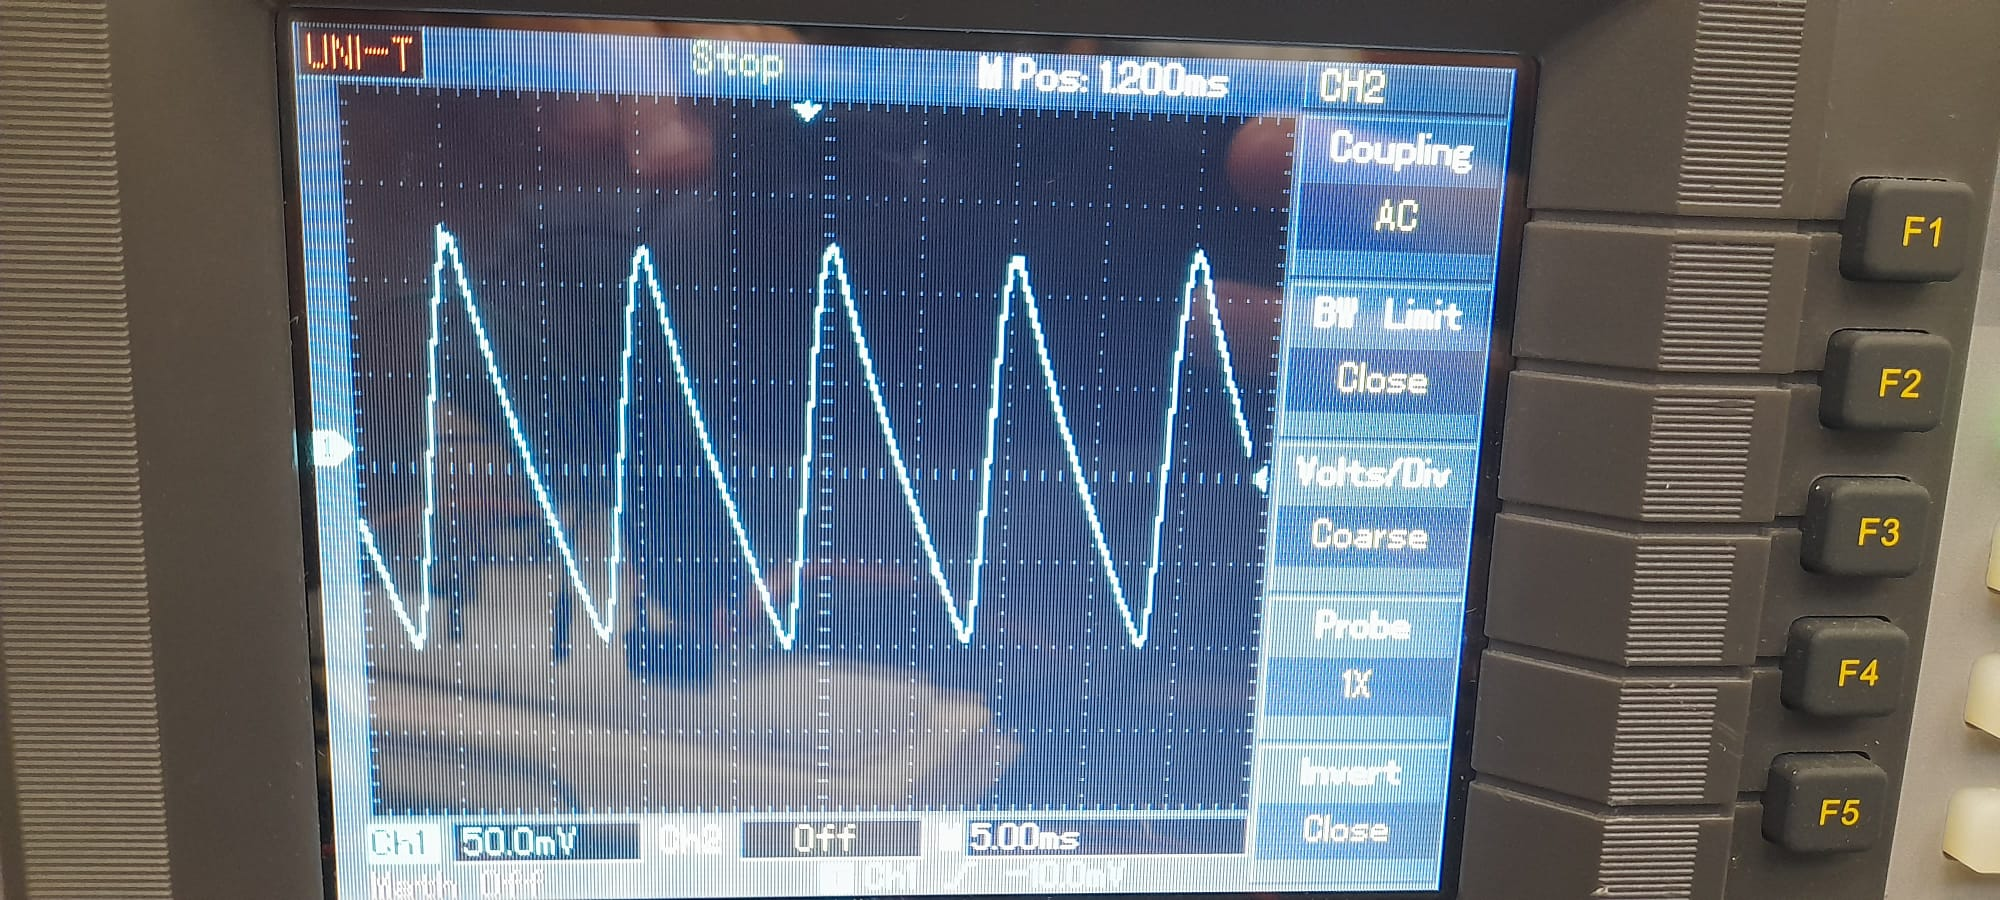
\includegraphics[width=6.3cm]{figures/ripple_lab_1N4007.jpeg} }}%
		\qquad
		\subfloat[\centering Medição - \textit{B250C2300-1500} \label{fig:rippleb250}]{{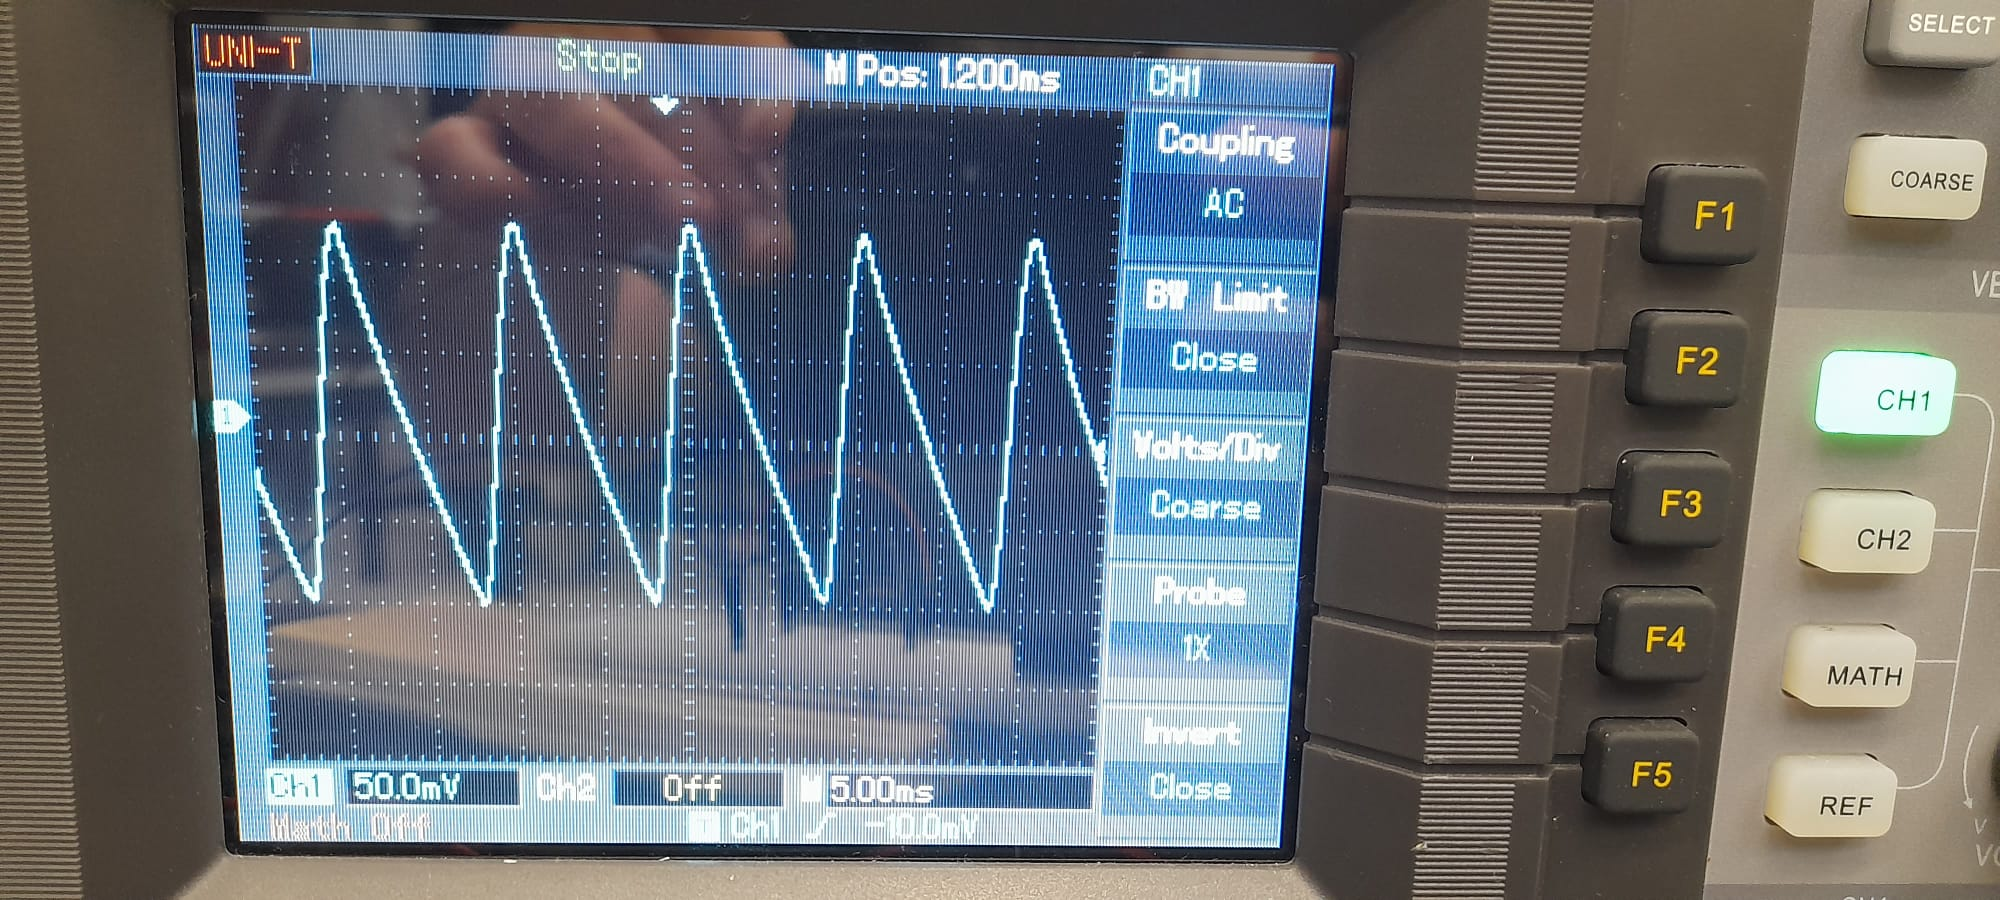
\includegraphics[width=6.3cm]{figures/ripple_lab_ponte.jpeg} }}%
		\caption{Medições práticas \textins{complementares} \textit{ripple}}%
		\label{fig:testesrippleOC}%
	\end{figure}

\begin{comment}
Outra dificuldade que contribuiu para justificar os erros obtidos — nomeadamente a discrepância no valor de \textit{ripple} calculado, dado que, devido ao aumento de $U_{Resistencia}$, seria de esperar um aumento do \textit{ripple}, conforme apresentado na Tabela~\ref{Table:testespontes} — está relacionada com as medições efectuadas no \acrshort{virtualbench}. A Figura~\ref{fig:distorcaoripple} mostra um exemplo de uma forma de onda adquirida com este equipamento, onde é visível a distorção do sinal de \textit{ripple} devido à presença de picos e ruído. Esta distorção pode comprometer a precisão da medição, dificultando a determinação rigorosa do valor real de \textit{ripple}. \textbf{Colocar uma imagem comparativa do osciloscópio para comparar as ondas? OPINIÃO PROF}
\begin{figure}[hbtp]
	\centering
	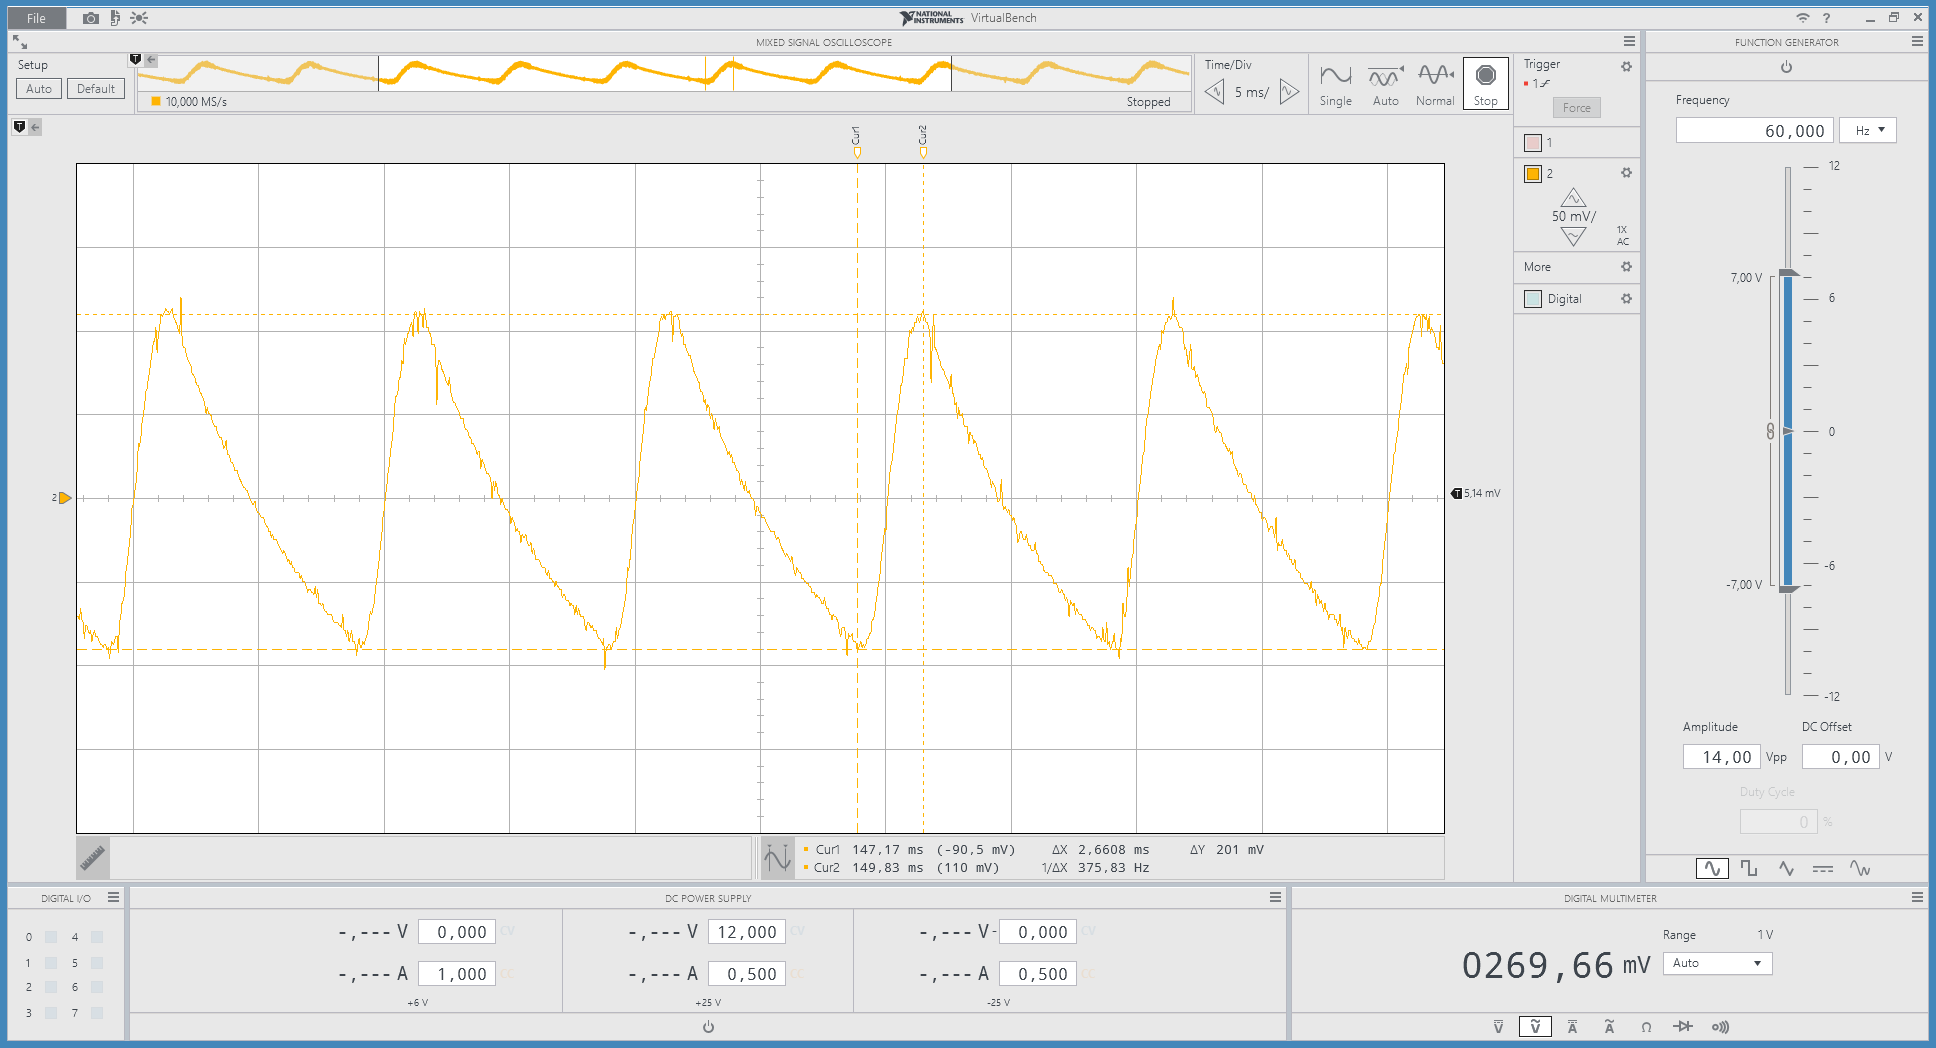
\includegraphics[width=0.7\textwidth]{figures/OC_RIPPLE_VB_1N4007.png}
	\caption{Distorção tensão \textit{ripple} \acrshort{virtualbench}}
	\label{fig:distorcaoripple}
\end{figure}
\end{comment}

Os resultados obtidos com o \acrshort{lare} encontram-se representados na Figura~\ref{fig:ripplelareonda}, onde é possível observar a forma de onda da tensão de saída, bem como o valor correspondente da tensão de \textit{ripple}. 

\begin{figure}[hbtp]
	\centering
	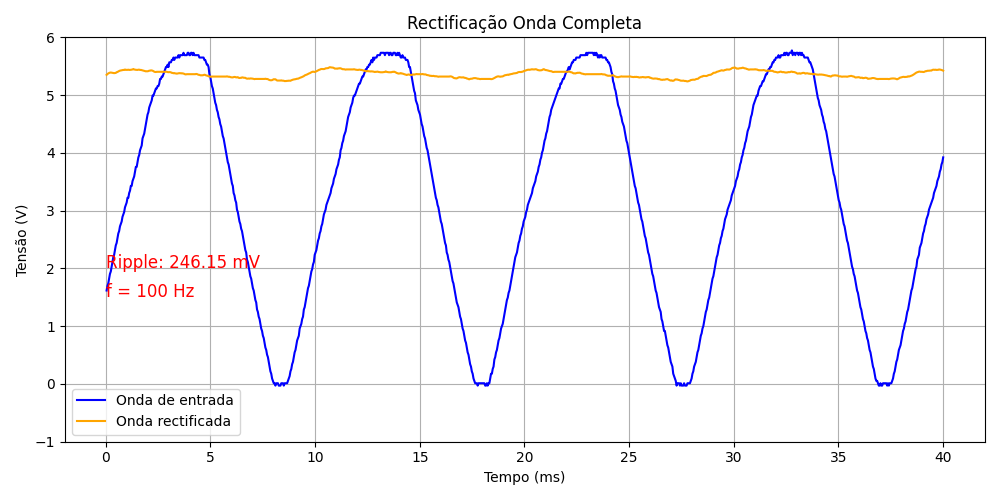
\includegraphics[width=0.6\textwidth]{figures/onda-completa.png}
	\caption{Tensão de \textit{ripple} no \acrshort{lare} - onda completa}
	\label{fig:ripplelareonda}
\end{figure}

É importante referir que, embora ambas as formas de onda (entrada e saída) tenham sido adquiridas com os mesmos parâmetros de configuração — nomeadamente, a mesma frequência de amostragem e tempo de aquisição —, os sinais não foram captados em simultâneo. Este procedimento foi necessário devido à configuração desta experiência, em que a ligação comum de massas entre a entrada do transformador e a saída do circuito impede a medição simultânea dos dois sinais com o \acrshort{virtualbench}, sob pena de provocar curto-circuito de massas. Assim, as medições tiveram de ser realizadas de forma sequencial, com reconfiguração dos relés entre cada aquisição. Ao reiniciar o osciloscópio, o sistema volta a aguardar pela condição de disparo (\textit{trigger}), a qual pode ocorrer em pontos ligeiramente diferentes do ciclo da onda. Esta diferença no instante inicial da aquisição introduz um desfasamento temporal aparente entre os sinais apresentados, que não deve ser interpretado como um desfasamento real entre os circuitos, mas sim como uma consequência natural da aquisição faseada.

O erro relativo associado ao valor obtido no \acrshort{lare} é inferior a \SI{5}{\percent}, o que é perfeitamente aceitável.

Os testes efectuados no \textit{multisim} com a ponte rectificadora constituída por 4 díodos \textit{1N4007} apresentam um valor de \textit{ripple} de \SI{201}{\milli\volt}, conforme representado na Figura~\ref{fig:ripplemultisim}. O erro relativo é de \SI{14.9}{\percent}, o que é aceitável, tendo em conta as condições de simulação, a distorção e ruído da onda e os componentes ideais utilizados, como é o caso, por exemplo, do condensador sem resistência série (ESR). Esta distorção pode comprometer a precisão da medição, dificultando a determinação rigorosa do valor real de \textit{ripple}. Tal como já referido na análise à rectificação de meia onda, a elevada tolerância do condensador electrolítico e as correntes baixas nos díodos são factores que também condicionam o erro relativo. Assim, as diferenças observadas são compreensíveis e enquadram-se dentro do esperado.

\begin{figure}[hbtp]
	\centering
	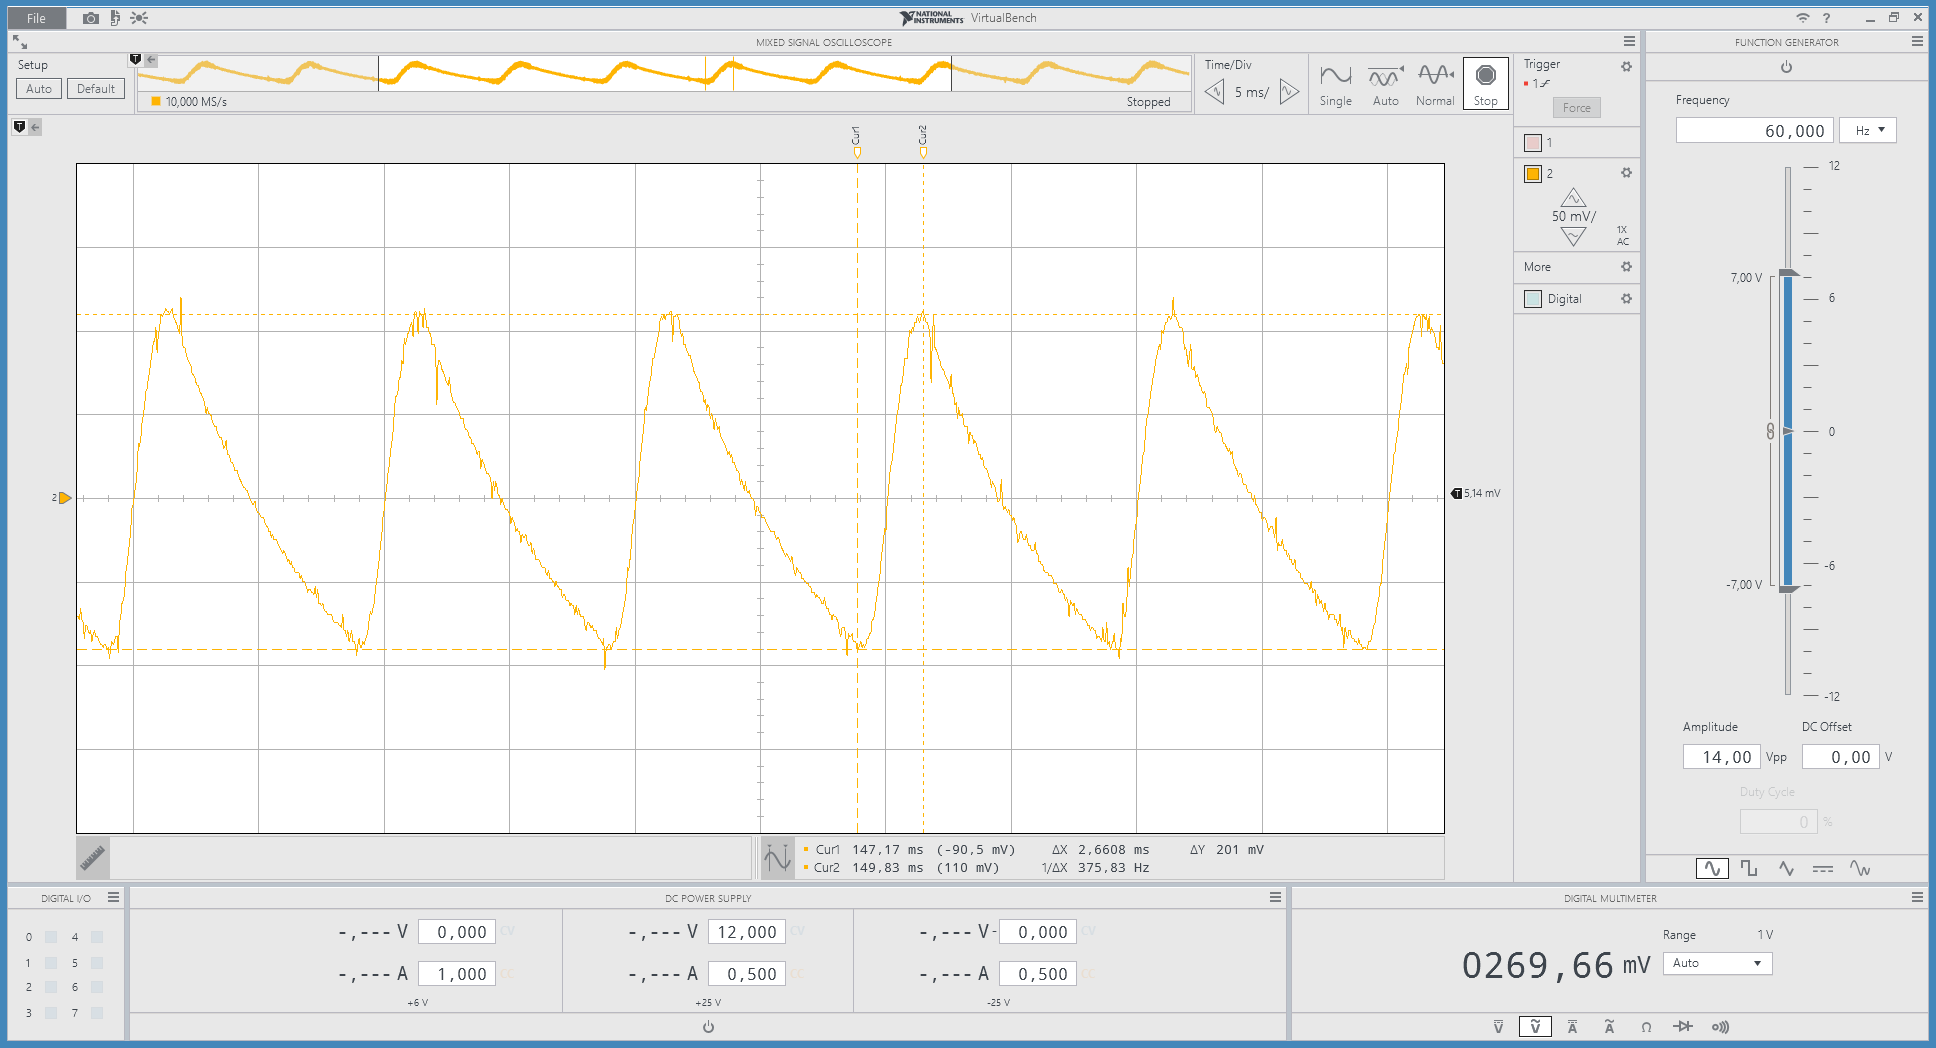
\includegraphics[width=0.5\textwidth]{figures/OC_RIPPLE_VB_1N4007.png}
	\caption{Tensão de \textit{ripple} - \textit{multisim} - onda completa}
	\label{fig:ripplemultisim}
\end{figure}

Comparando os resultados da tensão de \textit{ripple} entre os dois rectificadores e considerando os diferentes testes, verifica-se que, nas mesmas condições, a tensão de \textit{ripple} é superior no rectificador de meia onda, o que está de acordo com a teoria.


\section{Filtros}
\label{sec:resultados_filtros}
Estas duas experiências foram realizadas com o objetivo de estudar a resposta em frequência dos filtros $RC$, nomeadamente nas configurações passa-alto e passa-baixo, resultantes das diferentes configurações entre as resistências e os condensadores. Os utilizadores podem variar a frequência entre \SI{50}{\hertz} e \SI{80000}{\hertz}, analisando o comportamento da tensão de saída em função da frequência. A frequência de corte é calculada através da Equação \ref{eq:frequenciacorte}, sendo posteriormente comparada com os valores obtidos experimentalmente no diagrama de \textit{Bode}. Adicionalmente, a atenuação da tensão de saída pode ser determinada através da Equação \ref{eq:relacaoGanho}, ou expressa em \SI{}{\decibel} utilizando a Equação \ref{eq:relacaoGanhodB}.

\subsection{Resultados experimentais [filtro passa-alto]}
\label{sec:resultados_filtros_passaalto}
O circuito analisado será o filtro passa-alto, representado na Figura \ref{fig:filtro_pa} e configurado com $R=\SI{2.2}{\kilo\ohm}$ e $C=\SI{10}{\nano\farad}$. Os gráficos que se esperam obter estão representados na Figura \ref{fig:Bode_pa}. Para os restantes valores e configurações, os resultados poderão ser obtidos de forma análoga e a frequência de corte teórica é dada pela Equação \ref{eq:frequenciacorte}, sendo que o valor obtido é de \SI{7234.32}{\hertz}.

Os valores experimentais obtidos com o \acrshort{lare} relativamente à análise do digarama de \textit{Bode}, estão representados na Figura \ref{fig:fcBode}, sendo que o valor aproximado da frequência de corte é de \SI{7071.1}{\hertz}. O erro relativo é de, aproximadamente, \SI{2.26}{\percent}. Este valor é perfeitamente aceitável, tendo em conta a tolerância dos componentes utilizados, os erros de medição e aproximações.

\begin{figure}[hbtp]
	\centering
	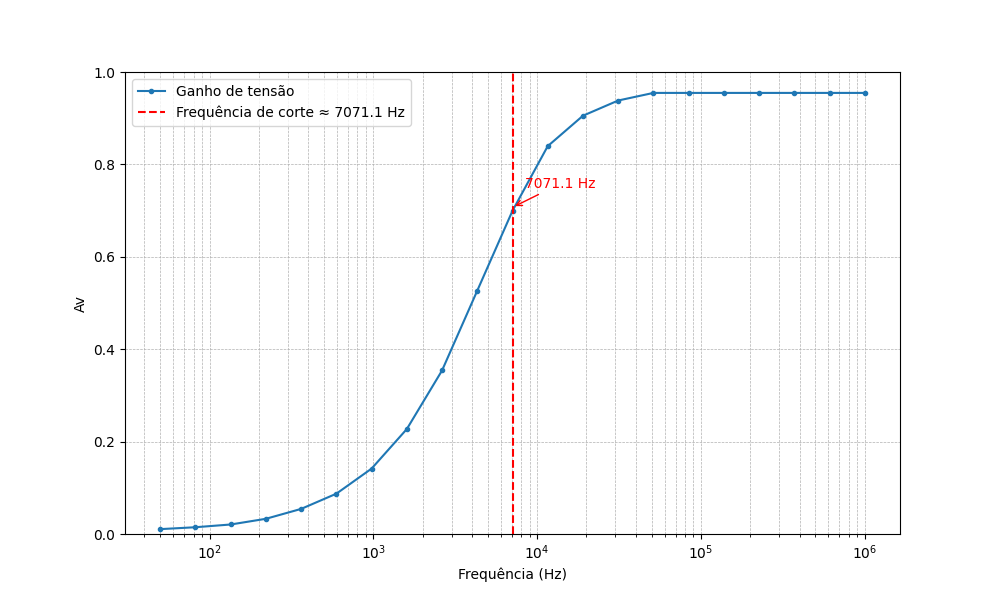
\includegraphics[width=0.5\textwidth]{figures/bode_hpf_fc.png}
	\caption{Frequência de corte - filtro passa-alto - Diagrama de \textit{Bode}}
	\label{fig:fcBode}
\end{figure}

Os resultados complementares obtidos com base na simulação efectuada no \textit{multisim}, já que não é possível gerar o diagrama de \textit{Bode} do circuito prático, representados na Figura \ref{fig:fcBodemultisim}, mostram que a frequência de corte é de \SI{7282.4}{\hertz}. O erro relativo é de \SI{0.67}{\percent}, o que é práticamente desprezável.

\begin{figure}[hbtp]
	\centering
	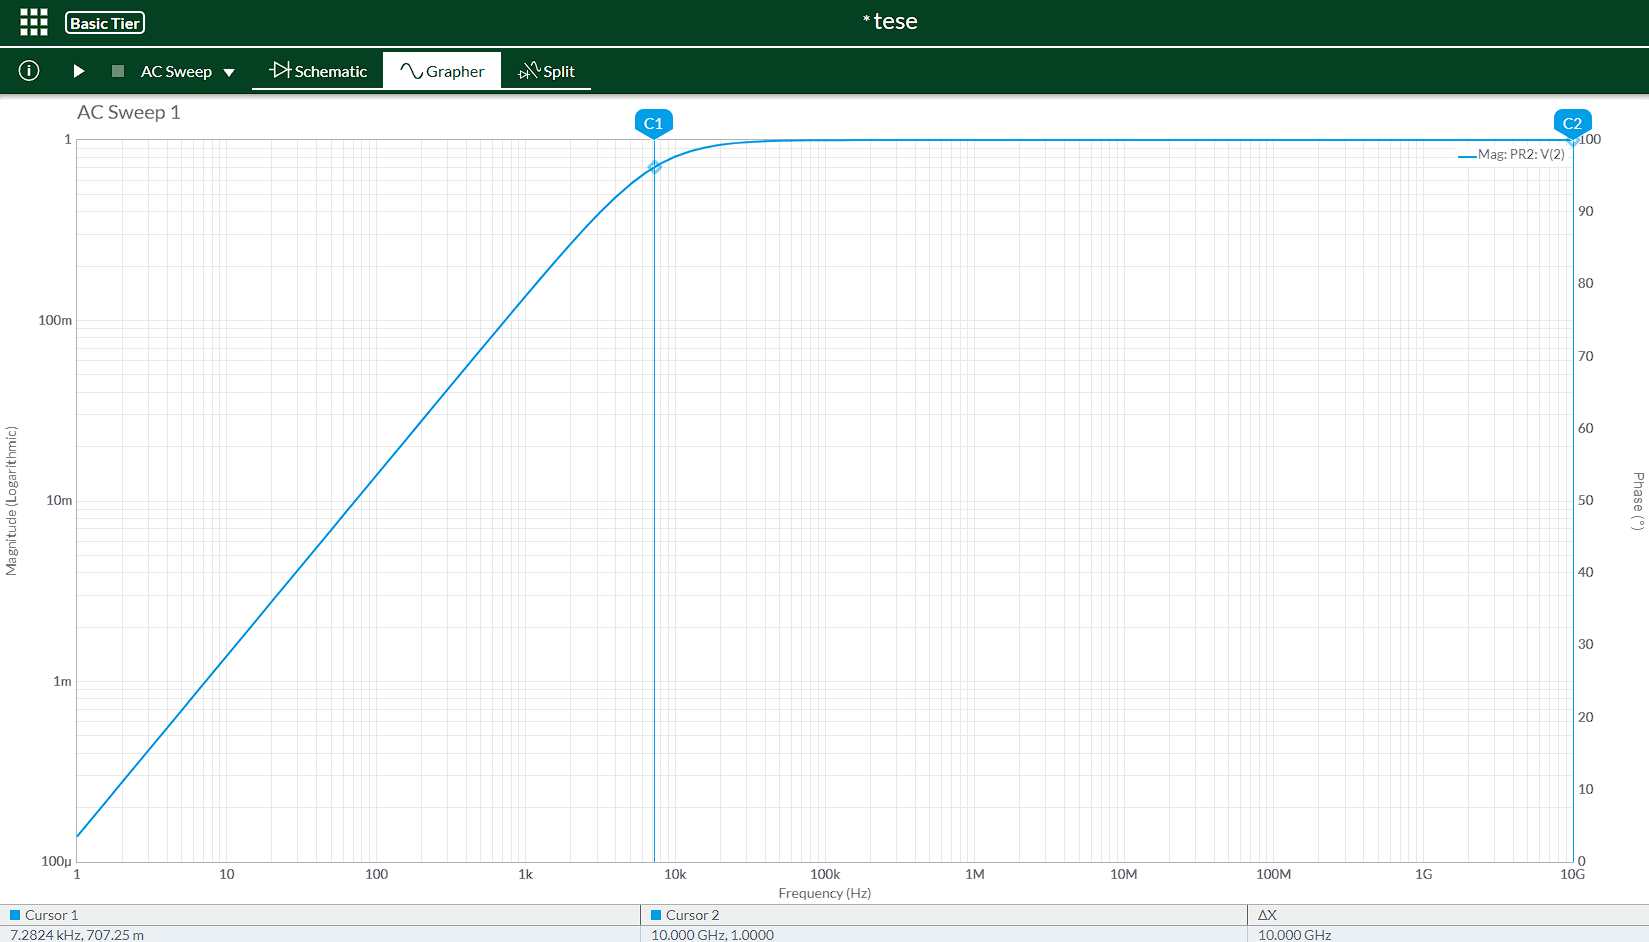
\includegraphics[width=0.6\textwidth]{figures/boda_HPF_fc.png}
	\caption{Frequência de corte - \textit{multisim} - Diagrama de \textit{Bode}}
	\label{fig:fcBodemultisim}
\end{figure}

O valor da frequência de corte também pode ser obtido através da análise dos gráficos que representam a relação entre a tensão de saída e a tensão de entrada. Como se pode ver pela análise da Figura \ref{fig:voutvinlare}, o ganho a altas frequências é práticamente unitário, estando em consonância com os valores obtidos no diagrama de \textit{Bode}, representado na Figura \ref{fig:fcBode}. 

\begin{figure}[hbtp]
	\centering
	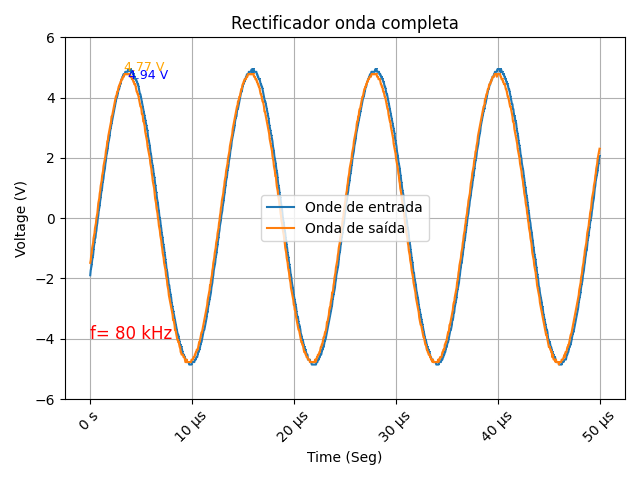
\includegraphics[width=0.6\textwidth]{figures/filtro_passa-alto.png}
	\caption{$v_{out}$ \textit{vs} $v_{in}$ \acrshort{lare}}
	\label{fig:voutvinlare}
\end{figure}

Comparando estes valores com os obtidos através do circuito prático, representados na Figura \ref{fig:realPA} e Figura \ref{fig:multisimPA} do circuito simulado no \textit{multisim}, verifica-se que os valores obtidos são práticamente iguais, podendo ser considerado, com segurança, que em ambos os casos o ganho de tensão é unitário. 

\begin{figure}[hbtp]
	\centering%
		\centering
		\subfloat[\centering Circuito prático\label{fig:realPA}]{{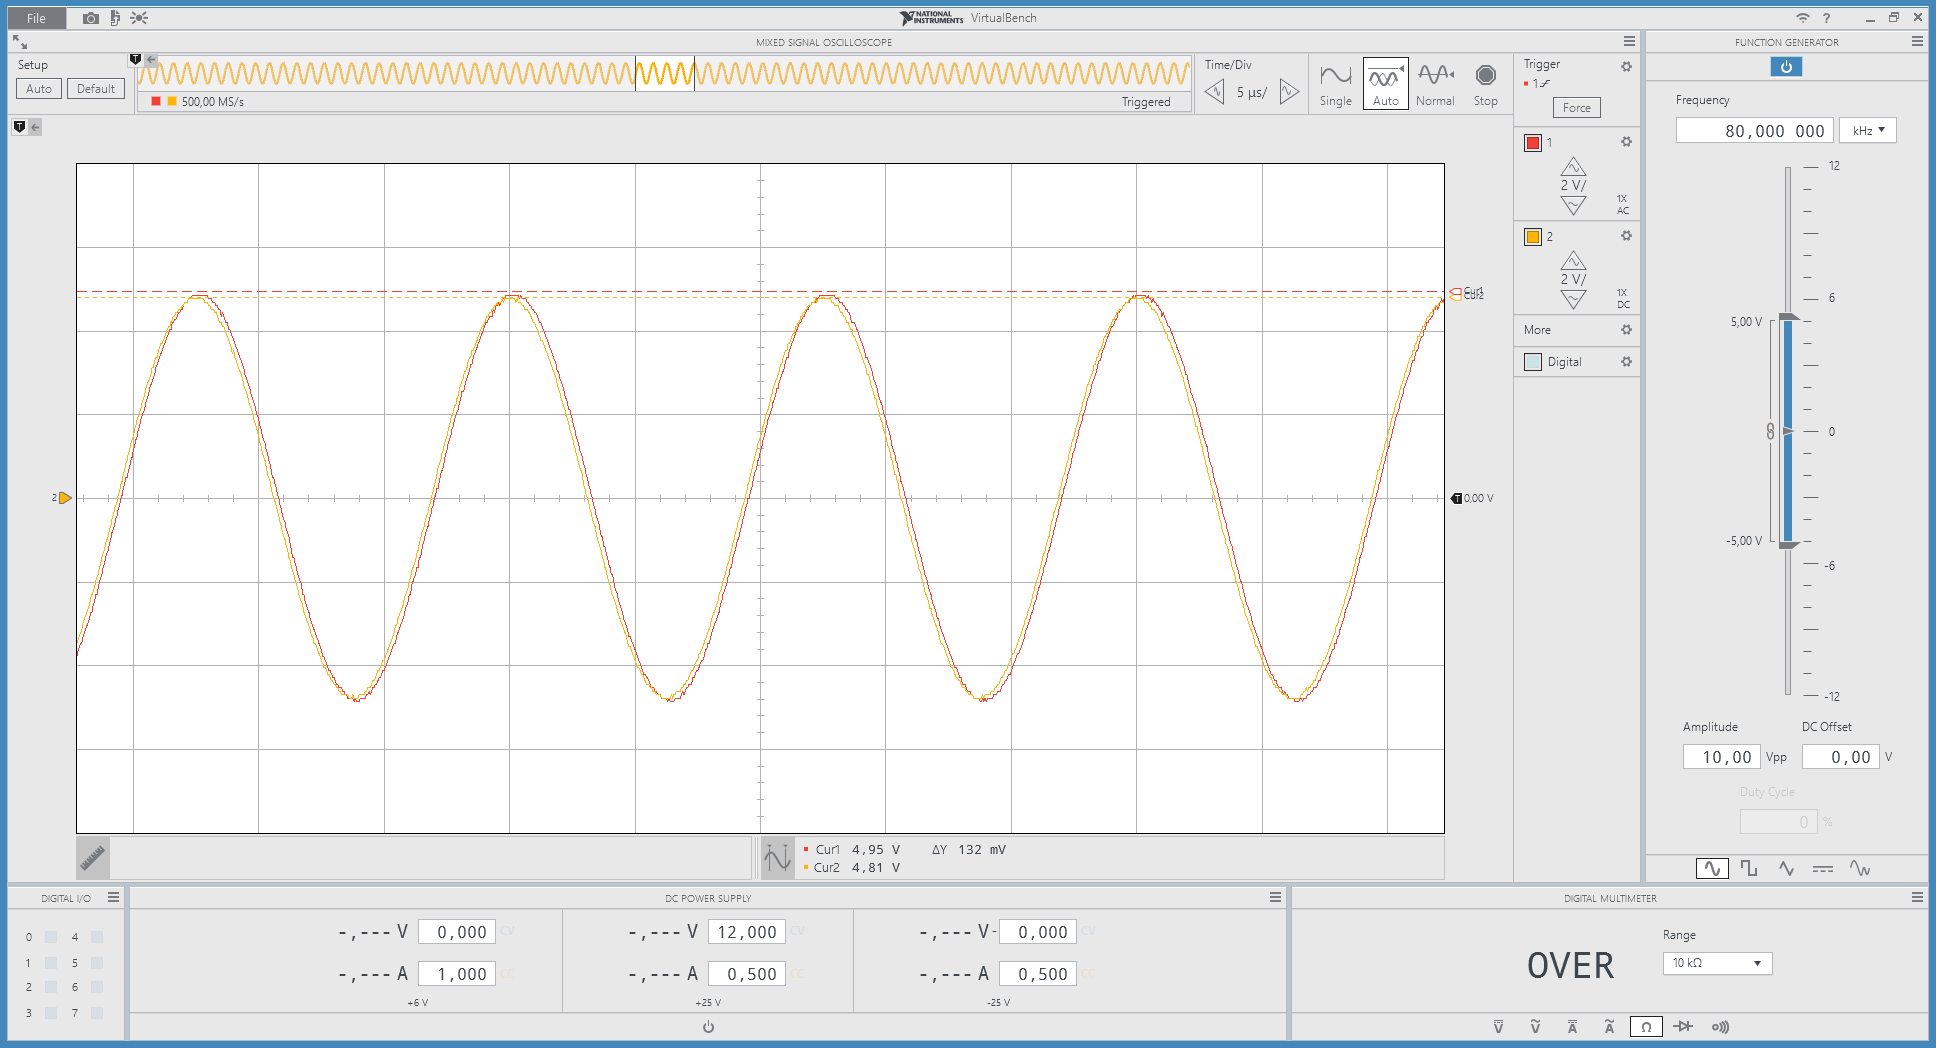
\includegraphics[width=6.3cm]{figures/PA_10nF2k2-80Khz.png} }}%
		\qquad
		\subfloat[\centering Simulação \textit{multisim}\label{fig:multisimPA}]{{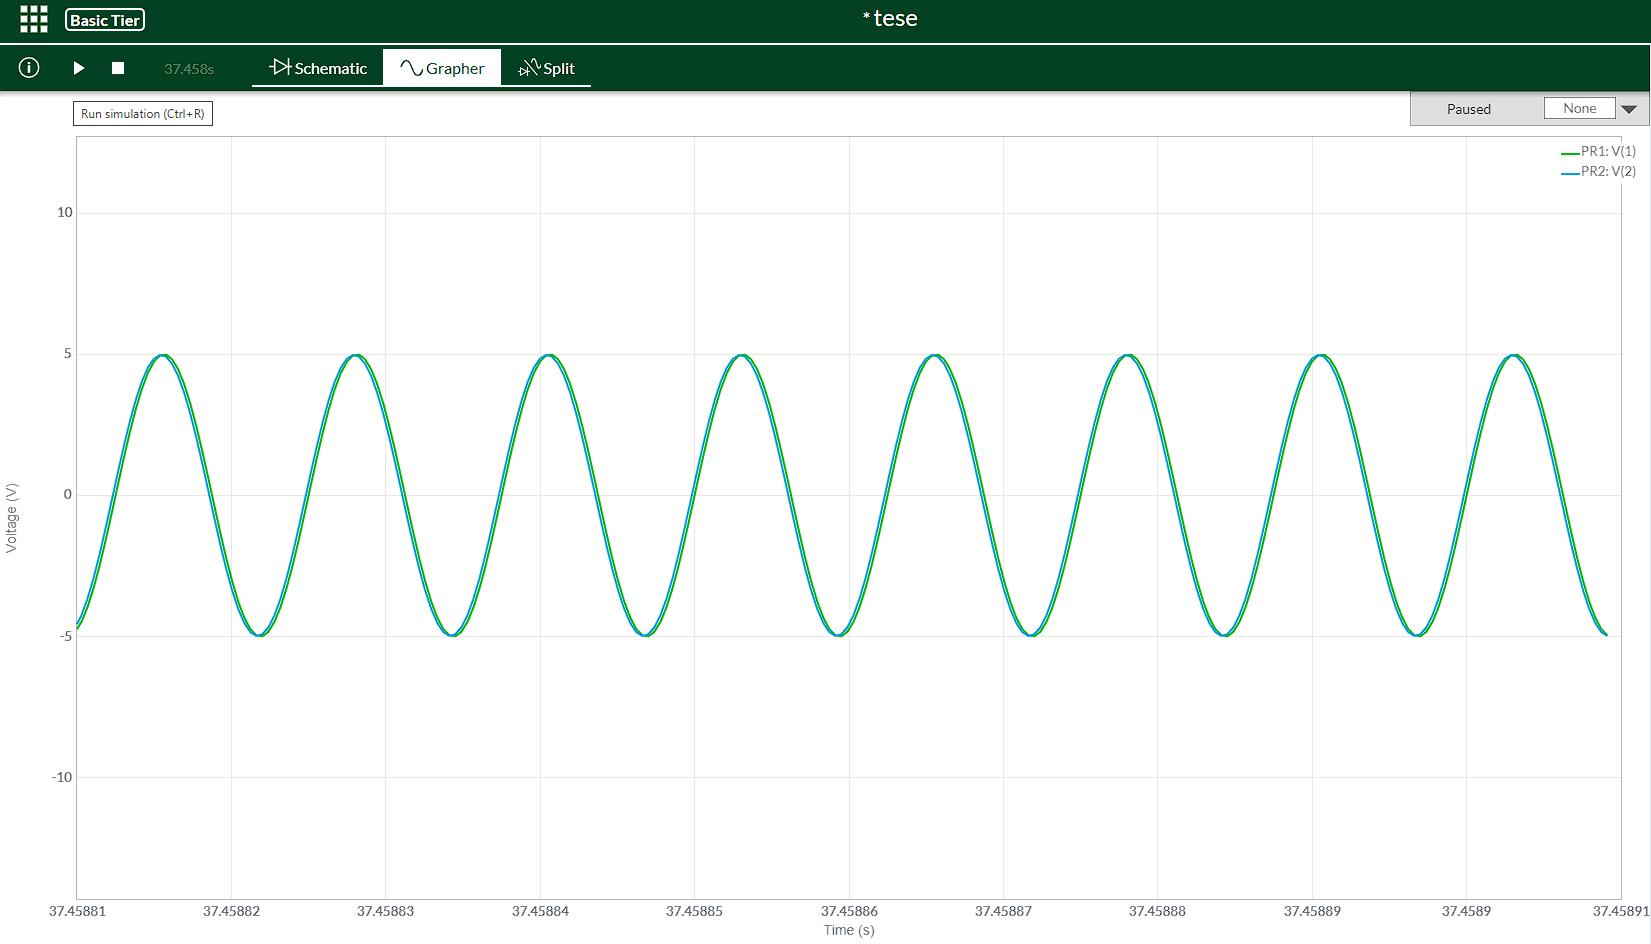
\includegraphics[width=6.3cm]{figures/boda_HPF_vout.png} }}%
		\caption{Valores práticos e simulados - $v_{out}$ \textit{vs} $v_{in}$}%
		\label{fig:simulacaoPA}%
	\end{figure}

Relativamente à análise da frequência de corte, representado na Figura \ref{fig:fcvoutlare}, o valor obtido para o \acrshort{lare} é de \SI{7230}{\hertz}, o que corresponde a um erro relativo menor que \SI{1}{\percent}.

\begin{figure}[hbtp]
	\centering
	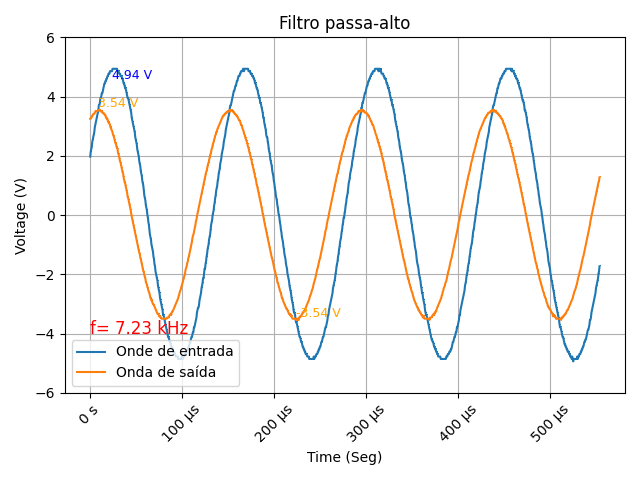
\includegraphics[width=0.6\textwidth]{figures/filtro_passa-alto_fc_LaRE.png}
	\caption{Frequência de corte - \acrshort{lare}}
	\label{fig:fcvoutlare}
\end{figure}

O circuito prático apresenta uma frequência de corte de \SI{7000}{\hertz}, com um erro relativo de \SI{3.24}{\percent}, enquanto a simulação no \textit{Multisim} apresenta \SI{7300}{\hertz}, com um erro ainda mais reduzido de \SI{0.9}{\percent}. Estes desvios podem ser considerados baixos e encontram-se dentro de margens aceitáveis, tendo em conta as limitações práticas do circuito real, como tolerâncias dos componentes, ruído e eventuais imprecisões nas medições. O valor obtido na simulação, por outro lado, está mais próximo do valor teórico, o que é expectável dado que os modelos usados assumem, geralmente, componentes ideais ou com parâmetros controlados.

\begin{figure}[hbtp]
	\centering%
		\centering
		\subfloat[\centering Circuito prático\label{fig:realfcvout}]{{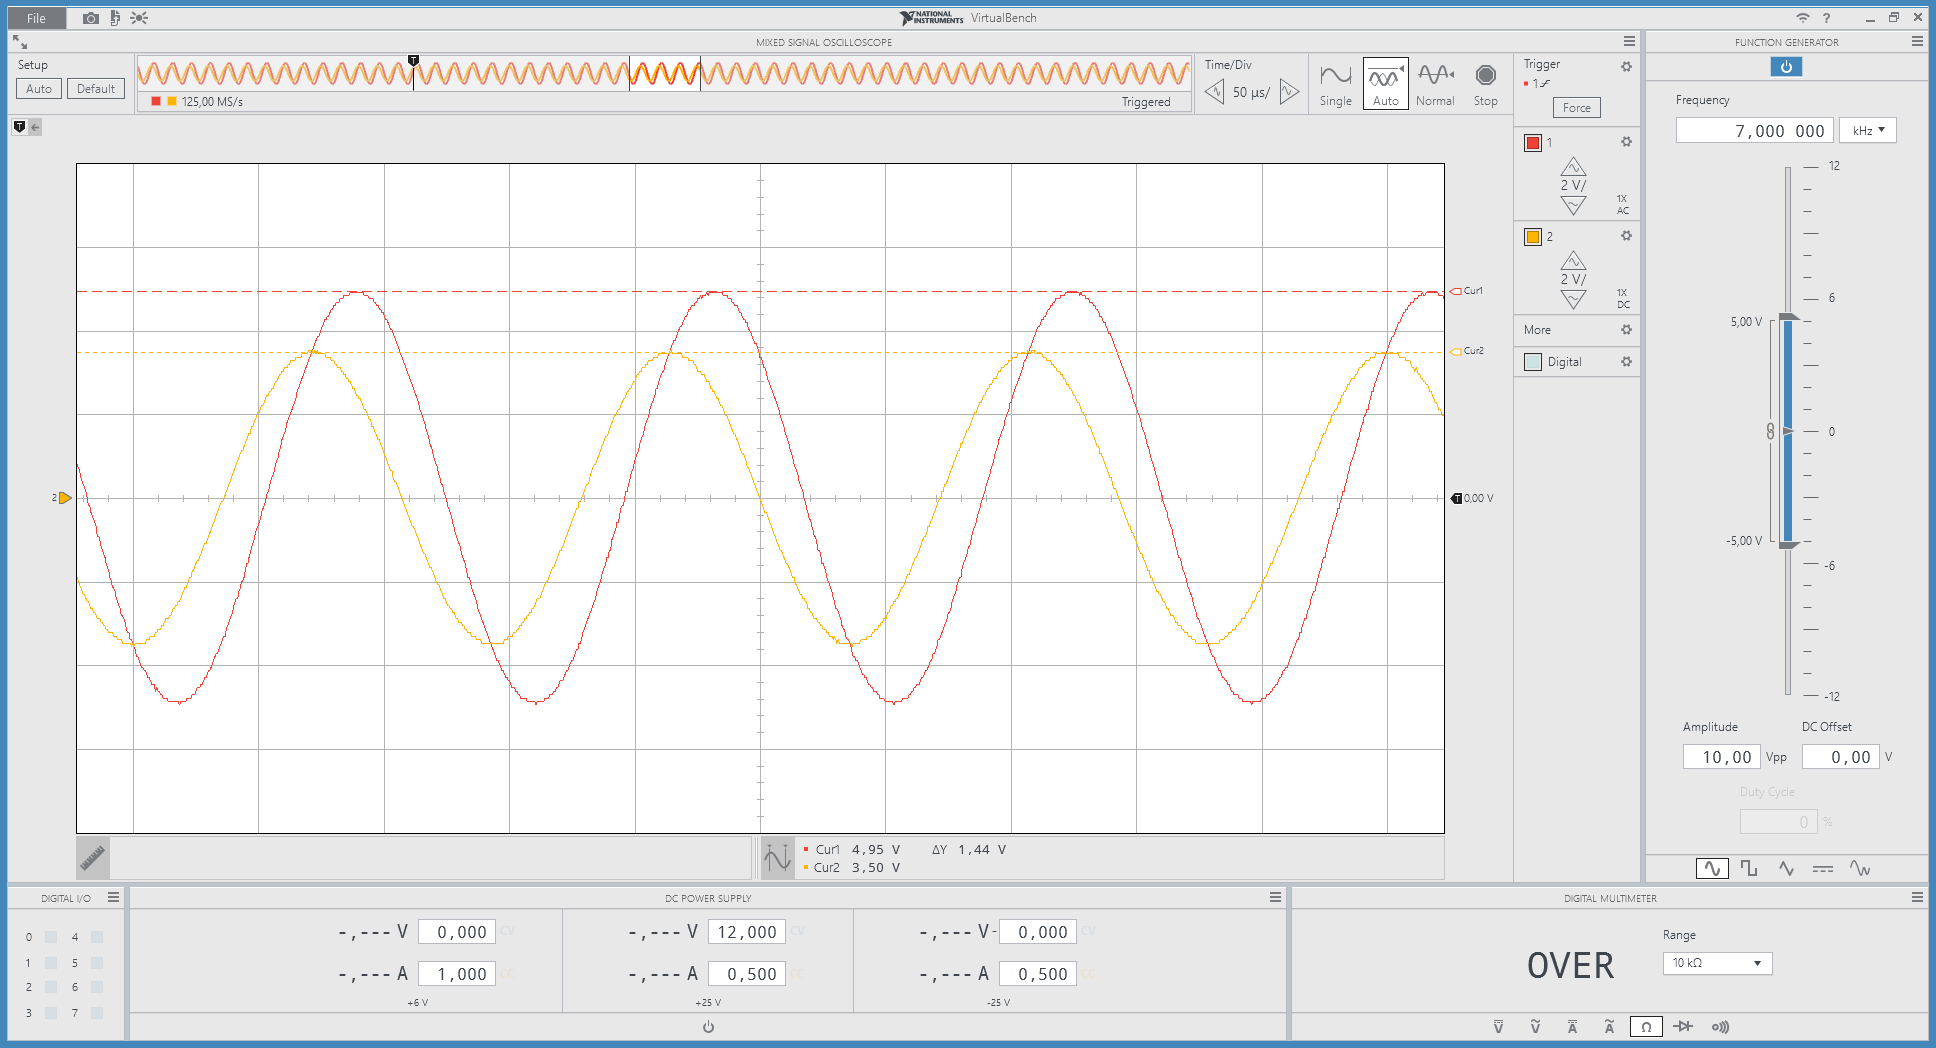
\includegraphics[width=6.3cm]{figures/PA_10nF2k2-Fc.png} }}%
		\qquad
		\subfloat[\centering Simulação \textit{multisim}\label{fig:multisimfcvout}]{{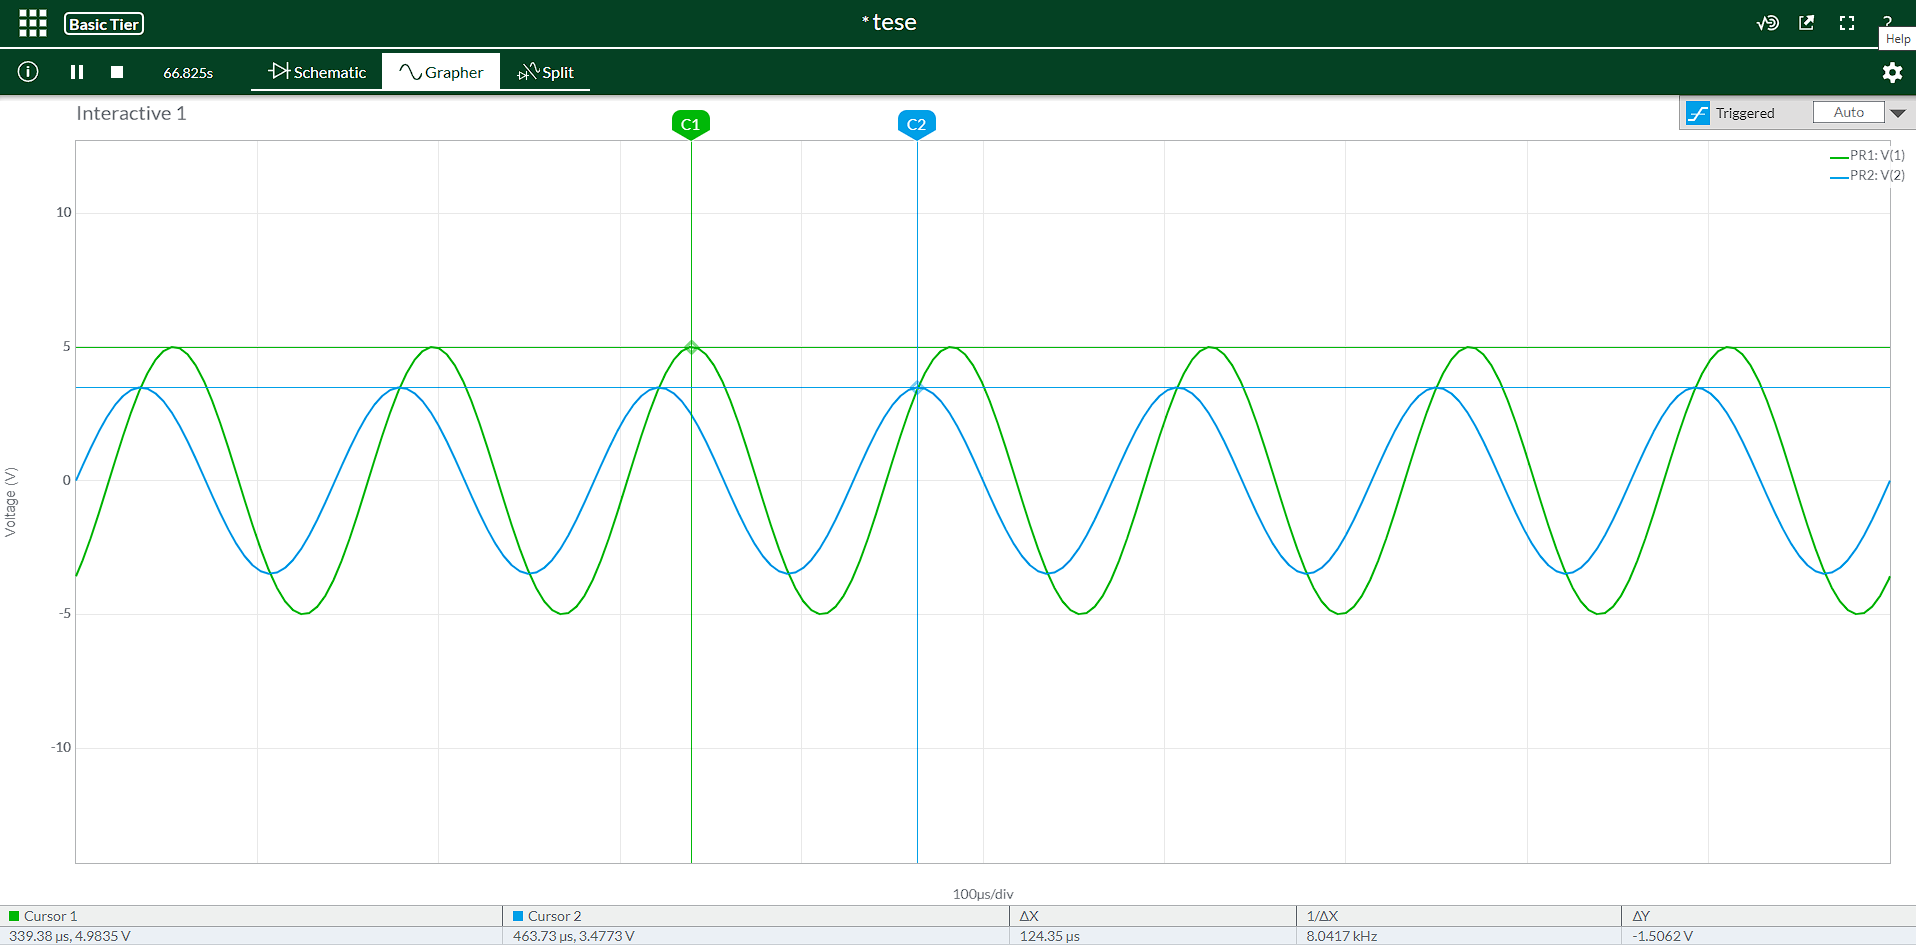
\includegraphics[width=6.3cm]{figures/boda_HPF_vout_fc.png} }}%
		\caption{Valores experimentais reais e simulados - frequência de corte - $v_{out}$ \textit{vs} $v_{in}$}%
		\label{fig:simulacaovout}%
	\end{figure}